\section{Background information: June 2015}
\subsection{Background} 
Some information about my project; yes, it is very cool.

\begin{table}[!htbp]
\caption{Results from \cite{Pascoe2014}}
\begin{tabular}{|c|c|}
\hline 
MU recruitment threshold & 3.3 $\pm$3.5\%MVC \\ 
\hline 
MU DC rate at recruitment & 9.0 $\pm$ 2.3 Hz \\ 
\hline 
Contraction duration & 21.4 $\pm$ 17.8 min (range 2.4-65.2 min) \\ 
\hline 
Contraction intensity & 5.5 $\pm$ 2.8 \%MVC \\ 
\hline 
DC rate during contraction & 10.6 $\pm$ 1.8 Hz \\ 
\hline 
\end{tabular} 
\end{table}

\subsection{Information} 
Information about my project showing again just how cool it is!

You really need to see it in its full glory. \lipsum[1]

\section{Protocol: July 2015}
\begin{itemize}
	\item Yup, this is the first step in my study.
	\item And this is the second
\end{itemize} 

\subsection{Protocol in detail}
\begin{enumerate}
	\item This is the real first step in my study, given that it is numbered `one'.
	\begin{itemize}
		\item This is the sub-step of step 1.
	\end{itemize}
\end{enumerate}

\subsection{Mock data}
Below is a figure of made-up data to help think about what the data may look like. 

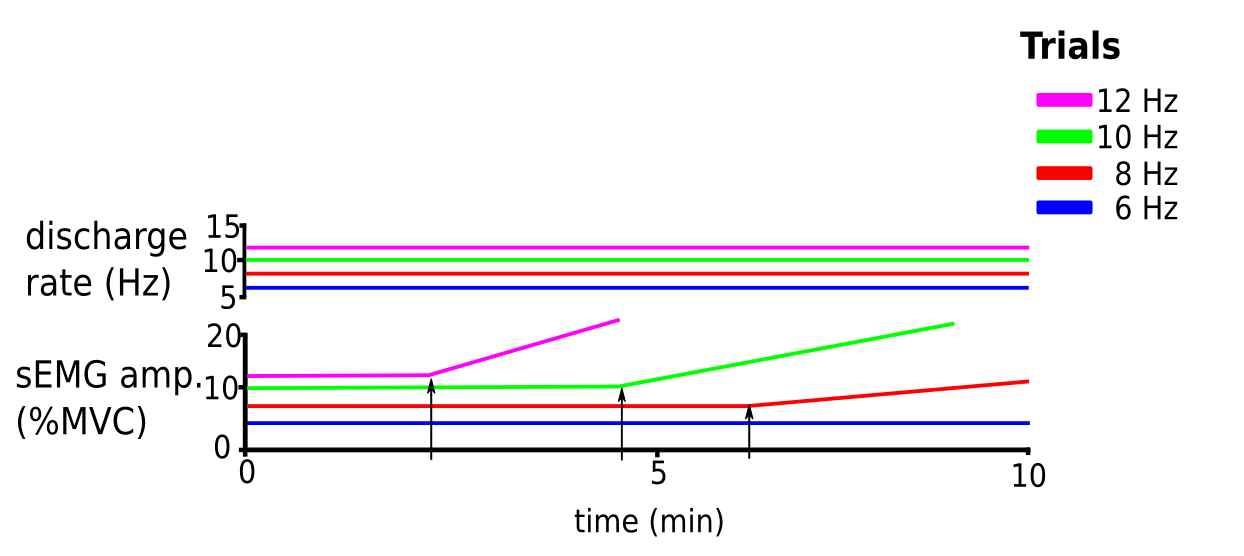
\includegraphics[scale=0.75]{./img/fake_data.png} 

\lipsum[1]